\documentclass{article} \usepackage[utf8]{inputenc} \title{} \author{Conrad Friedrich
\\ MCMP, LMU Munich \\ 500,000 words} \date{\today} \usepackage{setspace}

\usepackage{amsmath}
\usepackage{amssymb}
\usepackage{tikz}
\usepackage{ptolemaicastronomy}
\usepackage{ebproof/ebproof}
\usepackage[backend=biber,authordate,
ibidtracker=context,natbib,doi=false,isbn=false,url=false]{biblatex-chicago}

\addbibresource{/home/gilbert/Documents/bibliography/references.bib}

\newcommand{\nc}{\,\mid\!\sim\,}

\begin{document}

\maketitle
\section{Introduction}
This paper discusses Hans Rott' claim that principles of reasoning and belief
are subsumed under and derivable from what may be called principles of practical
reason and, in addition, Erik Olsson's reply. I argue that Olsson's criticism is
in part successful, but Sven Ove Hansson makes an even stronger point. To this
end, I first reconstruct a fragment of Rott's unifying framework and explain the
logical and epistemological systems involved. Then I look in detail at Olsson's
philosophical response. I conclude with a critical discussion.

The first part of this paper focusses on select elements of the formal systems
Hans Rott is unifying. I describe aspects belief revision theory, a study of
rational changes of belief, thus a theory situated between formal epistemology
and symbolic artificial intelligence. Next, I give an exposition of a certain
type non-monotonic logic, a type of logic that allows for defeasible inferences,
i.e. inferences which might be invalidated by further information. I then
present results already preceding Rott's work, in which both systems just
mentioned are shown to behave very similarly. Next, I give a brief description
of the theory of rational choice via choice functions, and finally describe how
Rott shows both belief revision and non-monotonic logic to be derivable as
choice functions.

The second part of this paper accepts the formal systems as given and evaluates
Rott's philosophical claim regarding the unity of practical and theoretical
reason. To this end, I look at Erik Olsson's criticism and discuss his arguments
in turn. I argue that Hansson's brief critique points to a deeper problem than
Olsson addresses, though.


\section{Belief Revision, Non-monotonic Logic, and Rational Choice}

\subsection{Belief Revision}
Belief revision if the form of the most prominent AGM
\parencite{alchourron85_logic_theor_chang} defines criteria for a rational agent
on how to update her beliefs when learning evidence. Crucially, this evidence
might be conflicting with what the agent already beliefs. For example, you are
about to pay your bill at a restaurant and, to your great surprise, there is no
money in your wallet \parencite[p.~48]{gaerdenfors88_knowl}.

In this framework, the agent's epistemic state is modeled by a set of sentences
from a standard propositional language \(\mathcal{L}\) closed under the boolean
operations \(\land, \lor, \neg, \rightarrow\). A consistent set closed under a
classical consequence relation \(\vdash\) is called \emph{belief set}. The three
key operations on a belief set are expansion, contraction and revision, each
with a single sentence. This sentence represents external input, e.g. the
content of a testimony of a trusted interlocutor. Expansion is only employed in
case the added belief is consistent with the belief set, such that it is a
special case of revision. Contraction and revision are interdefinable via two
postulates called Levi identity and Harper identity, defining contraction in
terms of revision and \emph{vice versa}, respectively.

Let us look then at the revision function from a sentence \(A\) and a belief set
\(K\), denoted \(K^*A\). What constitutes a rational revision? Following Quine`s
`maxim of minimum mutilation' \parencite[p.~72]{rott01_chang_choic_infer}, the
central postulates for belief revision aim at conserving as much as possible
from \(K\) in the new set \(K^*A\) while incorporating the new evidence
\(A\). \textcite{gaerdenfors88_knowl} describes six basic (minimal, elementary)
postulates, and two additional ones. In the interest of brevity, I will skip
listing them and refer to the numerous publications on these principles, e.g.
\textcite[p.~57]{gaerdenfors88_knowl, brewka97_nonmon},
\textcite{hansson17_logic_belief_revis}. As an example, the following postulates
states the success of a revision operation:
\[
    \label{eq:k2}
    \tag{$K^*2$} A \in K^*A
\]
This is supposed to prescribe that a rational revision operator always includes
the new belief in the belief set after updating. In General, the postulates are
designed to be intuitive and confirm to common sense (Cite). Importantly, the
postulates constrain the set of rational revision functions by way of logical
(set-theoretical) considerations, but do not necessarily determine a revision
uniquely \parencite[p.~53]{gaerdenfors88_knowl}.

To see this, let's consider an example. Suppose you believe that penguins are
birds, that birds fly, but penguins don't. We might represent the belief set as
\(K = Cn(\{ p \rightarrow b, b \rightarrow f, p \rightarrow \neg
f\})\),\footnote{Glancing over the fact that the beliefs are quantificational in
  nature. For the present purposes, the beliefs may be assumed to be about
  individuals, and that we have many such beliefs.} where \(Cn\) denotes a
classical consequence closure operator. We now learn that \(p\), i.e. that
Tweety is in fact a penguin. It is clear that when Tweety is a penguin, it can't
fly, even though it's a bird. The result of adding \(p\) to \(K\) is
inconsistent, so \(K\) has to be revised. How does the revised belief set
\(K^*p\) look like?

By the success postulate, we cannot drop \(p\). Since \(b \rightarrow f\) can be
assumed to be analytic, we won't drop that, either. Dropping either $b \rightarrow
f$ or $p \rightarrow \neg f$ leads to a revision satisfying postulates $K^*1 -
K^*8$. To decide between the two options in our formalism, we need additional
structure. There are a host of different such structures developed, prominently
\emph{partial meet contraction}
\parencite[p.~80]{gaerdenfors88_knowl} and 
\emph{epistemic entrenchment} \parencite[p.~86]{gaerdenfors88_knowl}. Both
are relational structures designed to prescribe a choice. Partial meet
contraction introduces a relation on maximal subsets of $K$ which don't  
imply $p$, while epistemic entrenchment orders sentences in K. To facilitate an
intuitive notion, I present a third `semantics' based on a sphere system by
\textcite{grove88_two_model_theor_chang} (also cf. \textcite[p.~83]{gaerdenfors88_knowl})
 
We define a set $W$ of possible worlds (which can be seen as maximal consistent
subsets of $\mathcal{L}$) organized into a set of concentric spheres $\mathcal{S}$ totally
ordered by $\subseteq$, such that $[K] = \{w \in W: w \models A \text{ for all } A \in
K\}$ is the minimal and $W$ the maximal element of $\mathcal{S}$.

Intuitively, the spheres rank the possible worlds by plausibility or normality,
with $K$, the belief set, ranked most plausible. Since $p$ is incompatible with
$K$, we have $[p] \cap [K] = \emptyset$. The idea is to revise $[K]$ such that
is only contains the most normal worlds satisfying $p$, i.e. worlds in the
$\subseteq$-minimal sphere \emph{and} in $[p]$. Compare Figure
\ref{fig:spheres1}, where $[K^*p] = S_1 \cap [p]$, such that $i \in [K^*p]$.

\begin{figure}[ht]
    \centering
    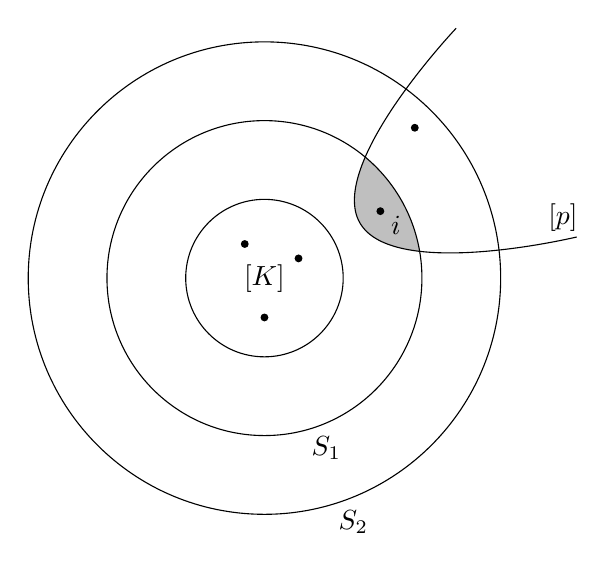
\begin{tikzpicture}[scale=1]
        % wider layers, pointier propositions
        \tikzset{layerwidth=1,innerfactor=0,
          proposition/.style={smooth,tension=1}}
        % fill the areas between three props and their innermost spheres
        % \sphereintersect{3}{\propositionplot{30}{3.3}{30}{4}}
        \sphereintersect{2}{\propositionplot{30}{2.3}{45}{4}}
        % \sphereintersect{1}{\propositionplot{30}{1.3}{60}{4}} draw the sphere
        % system
        \spheresystem[solid]{3}
        % draw the propositions \draw \propositionplot{30}{3.3}{30}{4};
        \draw \propositionplot{30}{2.3}{45}{4};
        % \draw \propositionplot{30}{1.3}{60}{4}; draw \psi (coordinates figured
        % out by trial and error) \draw plot[smooth,tension=1.2] coordinates
        % {(-1.5,3) (1.2,-1) (.8,2.3) (2.8,.7) (3,4)}; draw and label the center
        % world, spheres, and propositions
        % \filldraw circle[radius=.05];
        \node at (0,0) {$[K]$};
        \spherepos[fill]{30}{1}{circle[radius=.05]}
        \spherepos[fill]{120}{1}{circle[radius=.05]}
        \spherepos[fill]{270}{1}{circle[radius=.05]}
        \spherepos[fill]{30}{2.2}{circle[radius=.05]}
        \spherepos[fill]{45}{3.2}{circle[radius=.05]}
        \spherepos[fill]{22}{2.3}{node {$i$}}
        % \spherepos{-70}{1.8}{node {$S_1$}}
        \spherepos{-70}{2.8}{node{$S_1$}}
        \spherepos{-70}{3.8}{node {$S_2$}}
        % \spherepos{4}{4.3}{node {$\phi_1$} node at +(0,.5) {$\phi_2$} node at
        %   +(0,1) {$\phi_3$}}
        \spherepos{4}{4.3}{node at +(0,.5) {$[p]$}}
        % \spherepos{80}{4}{node {$\psi$}}
    \end{tikzpicture}

    \caption{Belief set $K$ in a system of spheres.}

    \label{fig:spheres1}
\end{figure}

How does this help with choosing between dropping $b \rightarrow
f$ or $p \rightarrow \neg f$? Depending on the agent's sphere system, either $i
\models p \land b \land f$ or $i \models p \land b \land \neg f$. Intuitively,
either the agent finds it more plausible that penguins fly or they
don't.\footnote{Note to self: what if $i_1 \models p \land f$ and $\i_2 \models
  p \land \neg f$, $i_1,i_2 \in K^*p$?} With the help of this additional
structure, then, we can uniquely define a revision.

Grove's sphere systems are provably `sound and complete' for revision functions
satisfying $(K^*1)-(K^*8)$, in a sense made precise by \textcite[][p.~84-85]{gaerdenfors88_knowl}.

\subsection{Non-monotonic Logic}

Non-monotonic logics define an conditional or a consequence relation that does
not satisfy monotonicity, i.e. additional evidence can demand a retraction of
previously drawn inference. Formally, the following inference is not valid for $\nc$. 
\begin{center}
    \begin{prooftree}
        \hypo{ \alpha \nc \beta } \infer1[(Mon)]{ \alpha \land \gamma \nc \beta}
    \end{prooftree}
\end{center}
I focus here on a type of non-monotonic logic called
\emph{preferential logic} developed by
\textcite{kraus90_nonmon_reason_prefer_model_cumul_logic}. KLM discuss a host of
conditions that the consequence relation can instead satisfy, and develop semantics for
salient sets of these conditions. For example, they introduce a weaker notion called 
cautious monotonicity:
\begin{center}
    \begin{prooftree}
        \hypo{ \alpha \nc \beta } \hypo{\alpha \nc \gamma} \infer2[(CMon)]{
          \alpha \land \beta \nc \gamma}
    \end{prooftree}
\end{center}
Important resulting logics are \textbf{C} (for cumulativity), \textbf{P} (for preferential), and \textbf{R}
(for rational), in increasing order of strength. 

Hans Rott shows that there is a close relation between the conditions
and the AGM postulates for revision
\parencite[p.~118,137]{rott01_chang_choic_infer}. Via the Gärdenfors-Makinson
identity, we can interdefine the two theoretical approaches:
\[ \beta \in K^*\alpha \text{ iff } \alpha \nc \beta \] for sentences
$\alpha,\beta \in \mathcal{L}$ and belief set $K$. Whether a sentence $\beta$
is included in the revision of $K$ by a sentence $\alpha$ can be seen as
validating a non-monotonic inference from $\alpha$ to $\beta$.

To spell this out a bit more, let's have a intuitive, brief look at a
(non-rigorous, simplified, finite)
version of the semantics for system \textbf{R} that \textcite{lehmann1992does}
define. A ranked model assigns each world $w \in W$ a rank $rk: W \rightarrow \mathbb{N}$
such that a relation $\prec$ on $W$ can be defined for all $w_1,w_2 \in W$:
\[
 w_1 \prec w_2 :\iff rk(w_1) < rk(w_2).
\]

Such a model validates a non-monotonic conditional $\alpha \Rightarrow \beta$ if
and only if the $\prec$-minimal $\alpha$-worlds are also $\beta$-worlds (compare
Figure \ref{fig:rank1} and \textcite[][p.~748]{ortner11_mechan_induc}).

\begin{figure}[ht]
    \centering
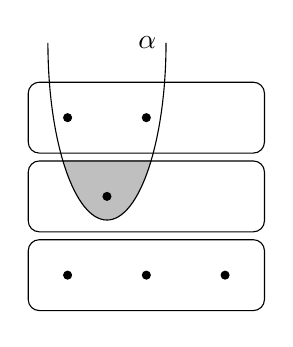
\begin{tikzpicture}
% \draw[help lines, thick] (0,0) grid (4,4);
\begin{scope}
\clip(0,0)rectangle(2,2);
\draw[fill,lightgray] (1.,3.5) circle [x radius=0.75, y radius=2.25];
\end{scope}\draw[rounded corners] (0, 0.1) rectangle (3, 1);
\draw[rounded corners] (0, 1.1) rectangle (3, 2);
\draw[rounded corners] (0, 2.1) rectangle (3, 3);

\draw[fill] (0.5,0.55) circle (0.05);
\draw[fill] (1.5,0.55) circle (0.05);
\draw[fill] (2.5,0.55) circle (0.05);
\draw[fill] (1,1.55) circle (0.05);
% \draw[fill] (2,1.55) circle (0.05);
\draw[fill] (0.5,2.55) circle (0.05);
\draw[fill] (1.5,2.55) circle (0.05);
% \draw[fill] (2.5,2.55) circle (0.05);

\draw (0.25,3.5) arc[start angle=180,end angle=360, x radius=0.75, y radius=2.25] node[left] {$\alpha$};

\end{tikzpicture}
\caption{A ranked model. The $\prec$-minimal worlds satisfying $\alpha$ are shaded.}
\label{fig:rank1}
\end{figure}

Now the similarity to the sphere system described in the preceding section is
not just superficial; we can in fact transform the ranked model into a sphere
system by setting $[K]$ to the $\prec$-minimal worlds, $S_1$ to the union of
$[K]$ and the $\prec$-minimal worlds of $W \ [K]$ and so forth. The semantics of
revision by $p$ are then very similar to validating a non-monotonic conditional
$\alpha \rightarrow \beta$. Note that we get this very neat correspondence of
the semantics not in all cases. In particular, the Grove sphere system requires
$(K^*1)-(K^*8)$, and ranked models are adequate for the strong logic \textbf{R}.

\subsection{Rational Choice}


\section{Erik Olsson's Critique}
\section{Discussion and Conclusion}
\nocite{rott01_chang_choic_infer,olsson03_belief_revis_ration_choic_unity_reason,gaerdenfors88_knowl,gaerdenfors94_nonmon_infer_based_expec,alchourron85_logic_theor_chang,makinson91_relat,sen93_inter_consis_choic,kraus90_nonmon_reason_prefer_model_cumul_logic,hansson17_logic_belief_revis,
  ortner11_mechan_induc,brewka97_nonmon} \printbibliography
\end{document}
